% !TeX root = ams_thesis.tex
\chapter{Interface Implementation}
\thispagestyle{fancy}

\section{Gesture Recognition}

The user interface for the control system uses the Kivy window management library. 
The UI uses ROS for its infrastructure, with the various components implemented as ROS nodes and communicating using ROS messages.
The user interface layer receives images from the robot arena overhead camera, and displays them, appropriately overlaid with buttons, to the user. 
The topmost layer receives user interactions in the form of contacts, and converts them to ROS touch events. The multitouch device emits a contact points that contain their location on the screen in cartesian coordinates, as well as identifiers for each contact.
Kivy's multitouch device handling adds other event information, including whether the contact is a double or triple tap, when the touch was last updated, and whether the event has ended (the finger has been lifted), how far the touch has moved since the last update, and whether the touch is associated with the activation of certain hardware, such as the mouse scrollwheel.
The majority of this metadata is not used. 
For process in later layers of the gesture recognizer, only the start, end, and update times, whether the event is a double or triple tap, the location of the point, and its identifier are passed as a ROS message. 
Button presses are also converted into ROS button messages which contain the time of the button press and the name of the button which was pressed. 

The user interface layer publishes touches, which correspond to single points of contact in both time and space as observed by Kivy. 
In order to collect points into strokes, a degree of cleaning of the input is needed. 
The primary source of error in strokes is stick-slip motion of the user's finger on the screen. 
When the user's finger slips, sometimes the screen regards the finger as having left the surface and returned quickly, breaking the stroke into two separate gestures. 
The ROS node destutter.py maintains a dictionary of lists of touches in the order that they arrived, indexed in the dictionary by the touch ID assigned by the user interface. 
As each stroke ends, it is compared to the other ended strokes. 
If the space in time and distance between the end of the recently completed stroke and the beginning of another stroke is small enough, the two strokes are merged into a single stroke. 
The parameters for the space and time thresholds for merging were set empirically, by intentionally causing stuttering contact with the screen and examining the reported time and distance between the beginnings and ends of contacts. 
At present, if the beginning and end of successive strokes overlap by less than 0.01 second, or are less than 0.15 second apart, they are considered candidates for merging. 
To be merged, candidates must also end and begin no more than 80 pixels apart. 
This value is approximately the width of a fingertip on the 3M screen, and is greater than the observed distance between stuttering strokes. 

Because a currently-ended stroke might be merged with a stroke that hasn't begun yet (that is to say, the user's finger might be in the air during the stutter of a stick-slip movement), strokes that have ended are not published unless there is no in-progress stroke that they could possibly be merged with. 
Every 0.2 seconds, the stroke cleaning node checks all the ended strokes against all the in-progress strokes. 
If the ended stroke's endpoint is closer than the distance threshold from the beginning of all of the active strokes, it could be merged with the active stroke. 
If the ended stroke is close enough to an active stroke's beginning to be considered, the time threshold is checked to determine if they could possibly be merged. 
If there is no active stroke that the current stroke could possibly be merged with, once that active stroke ends, then the current stroke could be published.
If the current stroke's end time is greater than the merge gap threshold in the past, then it is impossible for a new stroke to begin in time to be merged with the current stroke. 
Since there are then no active strokes it could be merged with, and it is impossible for a stroke to begin in time to merge with it, the stroke is then published. 

Strokes are recognized as gestures by a set of separate recognition modules. 
The initial design concept had been to have successive layers of recognition modules add more and more abstract information to the gestures, and arbitrate cases of ambiguity in gestures, but as the selected gesture set was intended to minimize ambiguity, this arbitration lead to additional complexity without any real gain in functionality or ability. 
It should also not be assumed that these gesture recognizers are the best method to perform the task, but they were sufficient during development, and investing significant time in improving them was beyond the scope of this project. 

If a gesture has fewer than 10 points or is fewer than 10 pixels across, it is classified as a tap. 
This classification is used because the user's finger distorts as it presses on the screen, and so can be registered as motion over a very small distance, even though the user was not dragging their finger. 
Gestures are classified into taps, lines, arcs, or closed shapes by the angle between the beginning and end of the gesture around the centroid. 
The thresholds for the angle around the centroid were \textless 1 radian to be classified as a circle, \textless 2.5 radians to be classified as an arc, and 2.5 radians or greater to be classified as a line. 
This sort of recognizer has problems with, for example, a circle drawn with a very tight scribble of points at one end. Placing the centroid in the center of the bounding box of the shape would result in it being recognized, correctly, as a circle, but the actual centroid as calculated from the points would be placed close to the dense knot of points at one end of the line, thus skewing the angle around the centroid. 

Gestures are then compared to information about the location of robots relative to the gesture on the screen to determine the meaning of the gestures. 
The gesture detectors are lasso and box selection, paths (lines that are not lasso or box selection), tap selection, tap as waypoint, and dragging of individual robots. 

The lasso gesture detector receives gestures from the gesture classifier and from the AprilTag detection node. 
If the gesture starts on a robot, it is considered a drag, where the user puts their finger on one robot, and drags from that robot to another location. 
If the gesture is not a drag, but is a closed shape, and there are robots located inside it, then it is a lasso selection. 
The lasso select gesture recognizer initially attempted to fit an oval to the points of the closed shape, but this approach was rejected because it does not work well if the user attempts to draw a concave polygon, such as a banana shape, in order to select some robots and not select others from a group of robots. 
Instead of using a fitted oval, the closed shape is treated as a polygon, and all robots inside the polygon are considered selected. 
If there are no robots, it is treated as a path, the generic classification for gestures with no other classification. 
If the gesture is not a drag, but is a line, it could be a box selection or a path. 
A box selection is a line whose bounding box includes at least one corner of an AprilTag. 
This requirement for inclusion, rather than including only AprilTags with their centers, or 3/4 of their points inside the bounding box, was chosen because the user survey on inclusion in selections that intersected the robot indicated that erring on the side of including partially-selected robots was preferable. 

If a path begins on a robot, it is the ``drag robot'' gesture, which is typically used by experiment participants to move an individual robot. 
The criteria for deciding that a path begins on a robot is the same as that used for deciding if a tap is intended to select a robot, as described below. 

Tap gestures are handled separately from strokes. 
If a tap gesture is on a robot, it is treated as selection of that robot. 
Taps that are not on a robot are treated as potential waypoints. 
For the purposes of making this distinction, a tap located within 80px of a robot is considered on the robot. 
The value of 80 pixels was chosen because it is the approximate width of a fingertip on the interface device, and so should be adjusted for devices of different resolutions. 
Alternatively, the mapping of pixels to real-world dimensions provided by the AprilTags could be used to calculate a conversion factor between the size of the screen and objects displayed on it in pixels and real-world meters, and the distance specified in terms of that conversion factor. 
Doubletap is the end-of-command gesture, and so is not treated as a waypoint or as a robot selection gesture. 

The gestures are then passed to the robot program generator, which adds them to a stack as they arrive. 
When the user terminates the gesture by either issuing an explict end-of-gesture double-tap, or by issuing a new selection gesture, which ends the previous command and begins a new one. 

\section{Translation Into Programs}
At the outset of this work, it had been hoped that there existed some form of transformation from the language defined by creating a formal description of an unambiguous subset of the user gestures to a potential language of robot behaviors. 
While the language of robot behaviors is itself not terribly well-defined, approaches such as the flavors of AutoMoDe and Supervisory Control Theory hint that the output language would likely be able to be represented as a DFA or PA, and so the resulting programs could then be amenable to analysis using a model checker such as PRISM \citep{KNP11}.

However, the user gesture language as defined by this work is actually quite vague, when it comes to commanding a robot to perform the expected actions. 
Alan Perlis has been quoted as saying ``When someone says `I want a programming language in which I need only say what I wish done,' give him a lollipop.'' , but regrettably, the user gesture language is just such a language, in part due to the design of the experiment \citep{PerlisYaleLolz}.  
Users were told to assume that the system was capable of understanding their orders, so they merely had to indicate what they wanted the system to do, and it would then do it. 
A system where the computer does what the user wishes done is more difficult to implement than the recipients of lollipops expect, because they rely on a large amount of \emph{a priori} information shared between the person issuing the command, and the system executing it. 

For example, in the box-moving task, the users would frequently move the robots to surround the box, and then move the robots to the goal area. 
However, one might expect that robot control programs would attempt to avoid obstacles, and so would just go around a box. 
Without the knowledge that boxes are acceptable to push against, no motion would occur, and the robots would in fact actively resist being steered to push the box. 
Even this knowledge shows the limitations of the gesture as a way of conveying a program to a robot.
The user data set does not have clear gestures for conveying that box-pushing is desirable, how to recognize the presence of a box, how to tell one box from potential other boxes, or how to convey that any particular object can be pushed, rather than just boxes. 
Instead, users assumed that the robots understood, as the user did, that the box was a thing that could be moved, and so did not have to be told.

Because the user gestures did not convey all of the information required to perform tasks, there is not a transformation that could operate purely on the user input to produce a program as output. 
Instead, the output program combines algorithms chosen by the system developer with parameterization from the user input. 
Because the system was intended to operate in a potentially unknown environment, the bug, dispersion, and occlusion-based transportation algorithms discussed in the previous section were used. 
If the environment were known, or communication were assumed to be reliable, other algorithms could be used. 
Indeed, the translation layer could be modified to switch algorithms based on the parameters of the swarm it is creating programs for and their environment. 

The development of the translation layer was performed in a manner similar to a compiler, which permitted the planning and other algorithms to be built into output programs by the translation layer. 
The input language was the user gestures, including which robots were selected and which user-specified paths were created. 
These inputs were used to parameterize the chosen algorithms, and the robots selected were used to determine the distribution of the resulting programs.
As a result, this work does not end up breaking away from iterative hand-coding, it just moves it from being done as a way of controlling the swarm, to being done as part of the creation of the control interface. 
For the motivating example from the introduction, urban search and rescue, this is acceptable, as it does not require the end user to program the swarm. 
It is also somewhat risky, as the resulting system may not have the flexibility that end users require. 

\section{Implementation Details}

User gestures arriving at the translation layer are stored in a stack until an end-of-command gesture arrives. 
The gesture sequence is then translated into a program that is parsed by the Lark parser library. 
Lark is an Earley parser, and so can parse all context-free grammars, although the current gesture language is not sufficiently complex to actually need this level of power. 
The resulting parse tree is then walked to generate GCPR programs that implement the algorithms described in Chapter \ref{chapter:Implementation_of_Swarm_Actions}.

Basic movement to points is implemented using the variant of TangentBug.
Path following and formation combines the basic movement to points with a sequence of GCPR instructions that implement a program counter, and set the goal based on the program counter. 
As each point is either reached or determined to be unreachable, the goal is advanced to the next point.
For motion along paths, the goals are set to points along the path, ending at the final goal. 
Formation allows the robot to stop at reachable points on the formation, but not unreachable points.  

Patrol also uses modified TangentBug, but instead of terminating when the program counter, and so the goal, reach the final position, the program counter and goal are reset to the start point of the patrol.  
As a consequence, the resulting program intentionally contains an infinite loop, but it can be interrupted by assigning a new program to the swarm. 

Dispersion is implemented using a minimalistic range sensor. 
Each robot can detect if there are other robots within a fixed range. 
If there are more than two robots in the range, the robot moves forward, avoiding obstacles. 
If there are exactly two robots in range, the robot stops. If there are less than two robots in range, the robot executes a U-turn and drives in a straight line, avoiding obstacles, until one of the other situations occurs. 
This algorithm is a GCPR implementation of the $\alpha$-algorithm of Winfield \emph{et al.}, and so shares its strengths and weaknesses  \citep{winfield2008modelling}.
Notably, the algorithm is not certain to prevent the separation of the swarm into subswarms that are not connected. 
More sophisticated programs, possibly using more communication, can prevent these issues, but since the requirement of the behavior is that the robots disperse, rather than that they maintain a particular level of network connectivity, there is no need for this particular implementation to enforce connectivity. 
Indeed, simply moving the robots to random locations uniformly selected would ``disperse'' them. 
However, selecting points would require foreknowledge of the area to disperse into. 
The $\alpha$-algorithm was chosen instead because it can operate in a previously unknown area, and because the resulting distribution looks even, visually. 
A randomly selected set of points from a uniform distribution may place two robots right next to each other, which, while ``uniform'' in a statistical sense, would appear uneven to the user, and not satisfy their intuitive understanding of dispersion. 
If dispersion in swarm robots continues to be a problem of interest, it is likely worth investigating the tradeoffs between speed of convergence, quality of dispersion, and user satisfaction with various methods. 

Manipulation was implemented as a simple version of occlusion-directed transport. 
If the robot is not near the target object, it attempts to move to the target object while avoiding obstacles, using the modified TangentBug algorithm. 
When the TangentBug algorithm detects that the goal is unreachable, because it is inside of the mobile object, the program switches to occlusion-based manipulation. 
The robot wall-follows around the object until a line from the robot to the goal intersects the object, and then pushes in that direction. 
While in this mode, the robot continually updates the direction of the goal, and switches between getting in position and pushing the object, as needed. 
As with the original occlusion-based manipulation, this algorithm is ignorant of obstacles on the opposite side of the object from the robot, and so can get stuck. 
However, as the system can accept a path for the object to be pushed on, the user can attempt to specify a clear path for the robots to move the object along. 

\section{Interpretation of Programs}

The robot algorithms were implemented as GCPR programs, and interpreted by a separate process for each robot. 

The GCPR interpreter starts with a single-line GCPR program that halts the robot, so all robots are stationary until they receive a new program. 
Programs are sent to each robot as ROS messages. 
When a robot receives a program, it begins executing it immediately. 
The GCPR interpreter runs at 100Hz, so 100 times per second, it evaluates the guards of each GCPR tuple, makes a list of all the commands whose guards evaluate to be true, and executes each command. 
The GCPR interpreter also implements a number of convenience methods such as is\_near\_front(), which returns true if any of the sensors on the front of the robot detect an object near them. 
The convenience methods are boolean, and intended to be used to create guards by boolean combinations of convenience methods with each other and with direct assertions about the sensors or other states of the robot. 
These methods are regarded as conveniences because they could be implemented as direct boolean statements about the sensor information of the robot, but the resulting GCPR statements would be extremely verbose. 

The interpreter also contains the implementations of the commands for the GCPR statements. 
The complexity of a command in GCPR is not limited. 
Because the system operates in the real world, at some point commands must result in changes to the state of physical actuators, and so the most atomic interactions might be simply the setting or clearing of given digital outputs. 
However, there is a trade-off between the complexity of the resulting commands and their utility to human users for writing programs. 
Carrying the complexity of the GCPR commands to the other extreme, the entire program could be implemented as the GCPR tuple (true, move\_to\_goal(), 1.0), which, under any condition, with probability 1.0, calls a command that moves the robot to the goal location. 
The resulting GCPR is quite compact, but the complexity is moved to the command implementation, where it becomes difficult to evaluate with formal methods. 

In seeking a balance between excessive conciseness in the expression of commands and excessive complexity in their implementation, the current implementation provides basic motion in lines, arcs, and rotation in place, and turning to face a given direction. 
There are also a number of methods to set and clear variables such as hit points, used in bug algorithms, and program counters, used in a number of GCPR implementations. 
All other complexity of the commands is contained in the GCPR statements which combine and control the motions, rather than in the motions themselves. 
For a future system, it may be more interesting to implement the swarm primitives suggested by McLurikin or Nagpal as commands themselves, and then allow more complex GCPR programs to use those commands \citep{mclurkin2004stupi, nagpal2004catalog}.
However, it then becomes incumbent on the implementer to ensure that the command implementations are correct. 
Having simple motions as commands eases correctness checking, as the motion will be performed, under the assumption that the motors are functional and the robot's path is unobstructed. 

If the commands are only outputs, the flow of information within the GCPR interpreter also becomes somewhat clearer. 
The sensor data is updated via callbacks triggered by ROS sensor information messages arriving, and is then used to evaluate the guards, and depending on which guards are true, commands are called to produce output. 
If the commands themselves are required to operate on sensor precepts, then the result of calling a command can change depending on the sensor information available when the precept is called.
Increasing the complexity of the commands also increases the time they take to execute, and so may present issues for operating the GCPR interpretation loop at 100Hz. 
The current implementation can very quickly set the desired motor speeds for a given motion and then return execution to the next command.
All of these factors argue in favor of keeping the GCPR commands close to motor primitives for the robot system, and keeping complexity in the control program in the GCPR code, rather than the commands. 

%\chapter{Compiler Verification}
%
%The design of a compiler which verifies that its output is correct What does it mean for a program to be correct? Free from things like assignment of variables to the wrong type, buffer overflows, off-by-one errors, etc. Does not mean that the program does what the programmer intended, just that it does whatever it does without errors. 
%Correctness is judged with respect to a specification. 
%Partial correctness - if an answer is returned, it is correct. 
%Total correctness - requires that program is partially correct and terminates
%No general solution to halting problem, needs specific proof per-program
%Compiler correctness shows that a compiler behaves according to its specification
%I don't currently have a language specification for the gesture language 
%
%One method of testing compilers is the operation of a fuzzer \citep{miller1990empirical}. A fuzzer, in the general case, generates input for programs that, while technically legitimate input, causes unexpected behavior such as program crashes. A fuzzer for compilers uses a description of the source language to generate programs that are considered valid under the description, and then attempts to compile them using the compiler. It can also attempt to generate programs that are deliberately incorrect, to test the ability of the compiler to accurately report errors, and to ensure that the compiler accepts all correct programs and no incorrect programs, as in \citep{bazzichi1982automatic}. 
%Because the internal structure of the compiler is not known, a generator cannot be certain that it causes all code paths in the compiler to be executed, but it can be certain that the generated test programs use all of the syntactical elements of the language, since all of the elements are described in the language specification. Interestingly, Bazzichi and Spadafora's work predates the use of the term ``fuzzer'' by 8 years, but clearly describes the same process.
%
%Translation validation \citep{pnueli1998translation}
%verifies compiled code against input code rather than attempting to verify that a compiler correctly translates all input programs.
%Verifies that the compiler correctly transforms a specific input program. 
%Needs:
% - A common semantic framework for the representation of the source code and the generated target code (probablistic finite automaton?)
% - A formal description of "correct implementation"
% - A proof method for verifying that one instance of the semantic framework (the output) correctly implements another one (the input)
%How is the IR not the common semantic framework?
%
%\section{Limitations}
%
%input semantics don't include way for user to set robot heading, might be useful for sensor overwatch

\section{Interface Testing}

In order to test the gesture recognition and translation components of the system, the recorded participant gestures from the gesture collection experiment were played back into the gesture interpretation pipeline. 
There exist two major ways that user gestures can fail to pass through the pipeline and result in a robot program. 
The first is that a gesture can fail to be recognized as what the user intended it to be. 
The gesture recognizers do not discard gestures as unrecognizable, but a stroke that does not meet the criteria for a drag, box selection, lasso, or any kind of tap is regarded as a path. 
If a user makes a selection gesture such as a box select, but the system does not recognize it as a box selection, the resulting sequence of gestures will not be able to be converted into a program. 
The second failure mode is that the user gestures are recognized correctly, but do not form a sequence that can be converted into a program. 

The first kind of failure, recognition failures, was detected by replaying the recorded user gestures and recording the output of the gesture recognizers in response to those gestures. 
The recognitions were then compared to the human coding for the user and task that generated the recorded input. 
Under the assumption that the human coding is correct, if the recognizer output differs, it indicates a defect in the recognizer. 

Detection of the second kind of failures, invalid gesture sequences, was detected by recording the reaction of the parser to the sequence of gestures created by the recognizers. 
It is possible for a sequence of gestures to create multiple parse attempts, by having, for example, a selection and path gesture followed by a second selection and path gesture.
The second selection terminates the first command and begins the second, and so the first parse attempt operates on the first selection and path, and the second parse attempt operates on the second selection and path. 
In cases where a gesture sequence resulted in multiple parse attempts, each parse attempt was treated as a separate trial, rather than allowing one failure to cause the entire task to be treated as a failure.  

Due to a hardware misconfiguration during the user test, multitouch contact points were only recorded during the first thirty of the human subject tests. 
For those thirty tests, any example gestures that the participant made were removed to prevent failures caused by the participant proposing alternative methods during a sequence of gestures, and so creating redundant gestures within the sequence. 
As discussed above, a gesture to end the command was required in cases where a new command did not end the previous one, and so each sequence of user gestures had a end-of-command gesture added to its end. 
Any end-of-command gestures that already existed in the gesture set were removed. 
The double-tap gesture performed on empty areas of the screen was chosen as the end-of-command gesture. 
Double-tap as selection was 7.3\% of the selection gestures, but its relative scarcity as a proportion of all gestures made it a good candidate for reservation for this purpose. 
Triple-tap is even more rarely used, and for that reason might have been a better option, but it is also more difficult to perform, which is a poor quality to have in a gesture that will be used at the end of almost every gesture sequence. 

Not all of the participants made gestures that would be expected to be recognized by the gesture recognizers. 
The implemented recognizers recognize box selection, lasso selection, tap selection (taps on robots), tap to set waypoints (taps on empty space), and drawn paths. 
As discussed above, the other functions had limited agreement between users, and so were implemented as buttons on the UI. 
Because user UI interactions were in various locations around the screen, they are not able to be directly converted to UI interactions with the interface as implemented. 
However, as UI interactions only constitute 3.4\% of the recorded interactions, this is not a large loss. 

Tasks where the user interactions fell outside of what the UI would be expected to recognize serve as negative examples.
They are unlikely to be correctly recognized, and so should not form acceptable sequences of commands. 
Despite the fact that this constitutes a failure, it is a desirable result, because if they are recognized and converted to robot programs, they are unlikely to accurately capture the user's intent. 

\subsection{Causes of Failed Recognition}

The gesture recognition elements of the user interface were not the primary thrust of this research, and so were primarily implemented in order to be able to provide gestures to the gesture compiler to attempt to generate programs. 
The effort to implement gesture recognition from scratch was undertaken because at the time, it was felt that collecting, assessing, and potentially training available gesture recognition systems was likely to take more time than implementing a simple recognition pipeline. 
It is difficult to assess the percentages of correct gesture recognitions as opposed to incorrect ones, as the ground truth data, the coding of the gesture experiment data by human coders, uses different categories for describing some of the gestures than the recognition system was developed to target. 
For example, a pinch gesture is frequently recognized as two drag gestures. 
In the single robot case, for the task of bringing the robots together in a group two robot drag gestures would bring the robots together, and so have the desired result. 
However, the recognition is still incorrect, as the gesture was a pinch, which the recognizers do not recognize because it is not a part of the gesture language. 
Similarly, the coding does not distinguish between drags starting on a single specific robot and drags starting within the robot swarm, although their context of other actions frequently makes the user intent clear. 
The recognition pipeline does distinguish drags starting on a robot from drags starting anywhere else, but because of a threshold in how close the start point has to be to the robots being on it, a drag that visibly does not start on a robot (and so may be coded as a non-robot drag) could still be recognized as a robot drag because it was close enough. 
However, despite these difficulties, some causes of failed gesture recognitions were sufficiently common to merit description below. 
%May they serve as a warning to others.  

There are a number of causes of failed recognition of gestures when the recognizers are provided with recorded participant inputs from the experiment. 
One cause is that the gesture made by the user is simply not one that the gesture recognizers can correctly recognize, and so any recognition they generate is incorrect. 
Because the pinch gestures and the 5-fingered scattering motion used to disperse the swarm by some participants are not implemented in the gesture recognizers, the pinch gesture is usually recognized as either two separate paths, or as two attempts to drag robots, or one of each. 
The 5-finger scatter is similarly recognized as 5 separate gestures, which may be paths if they are not over robots, or gestures to drag individual robots if they are. 

When participants made gestures that had broad contact areas, the multitouch screen rendered them as ladder-like lines of nearby points. 
In figure \ref{recogniser_fail_1}, the parallel lines of green points, especially visible on the left side, are points reported by the multitouch screen. 
They do not, however, represent the location of the user's fingers.
The user was using two fingers, located close to each other, to make the two arcing gestures visible in the data. 
Because the two points were located too close to each other to be reliably detected as separate points, the screen reported a single, interpolated location instead of the location of each fingertip. 

\begin{figure}
	\centering
	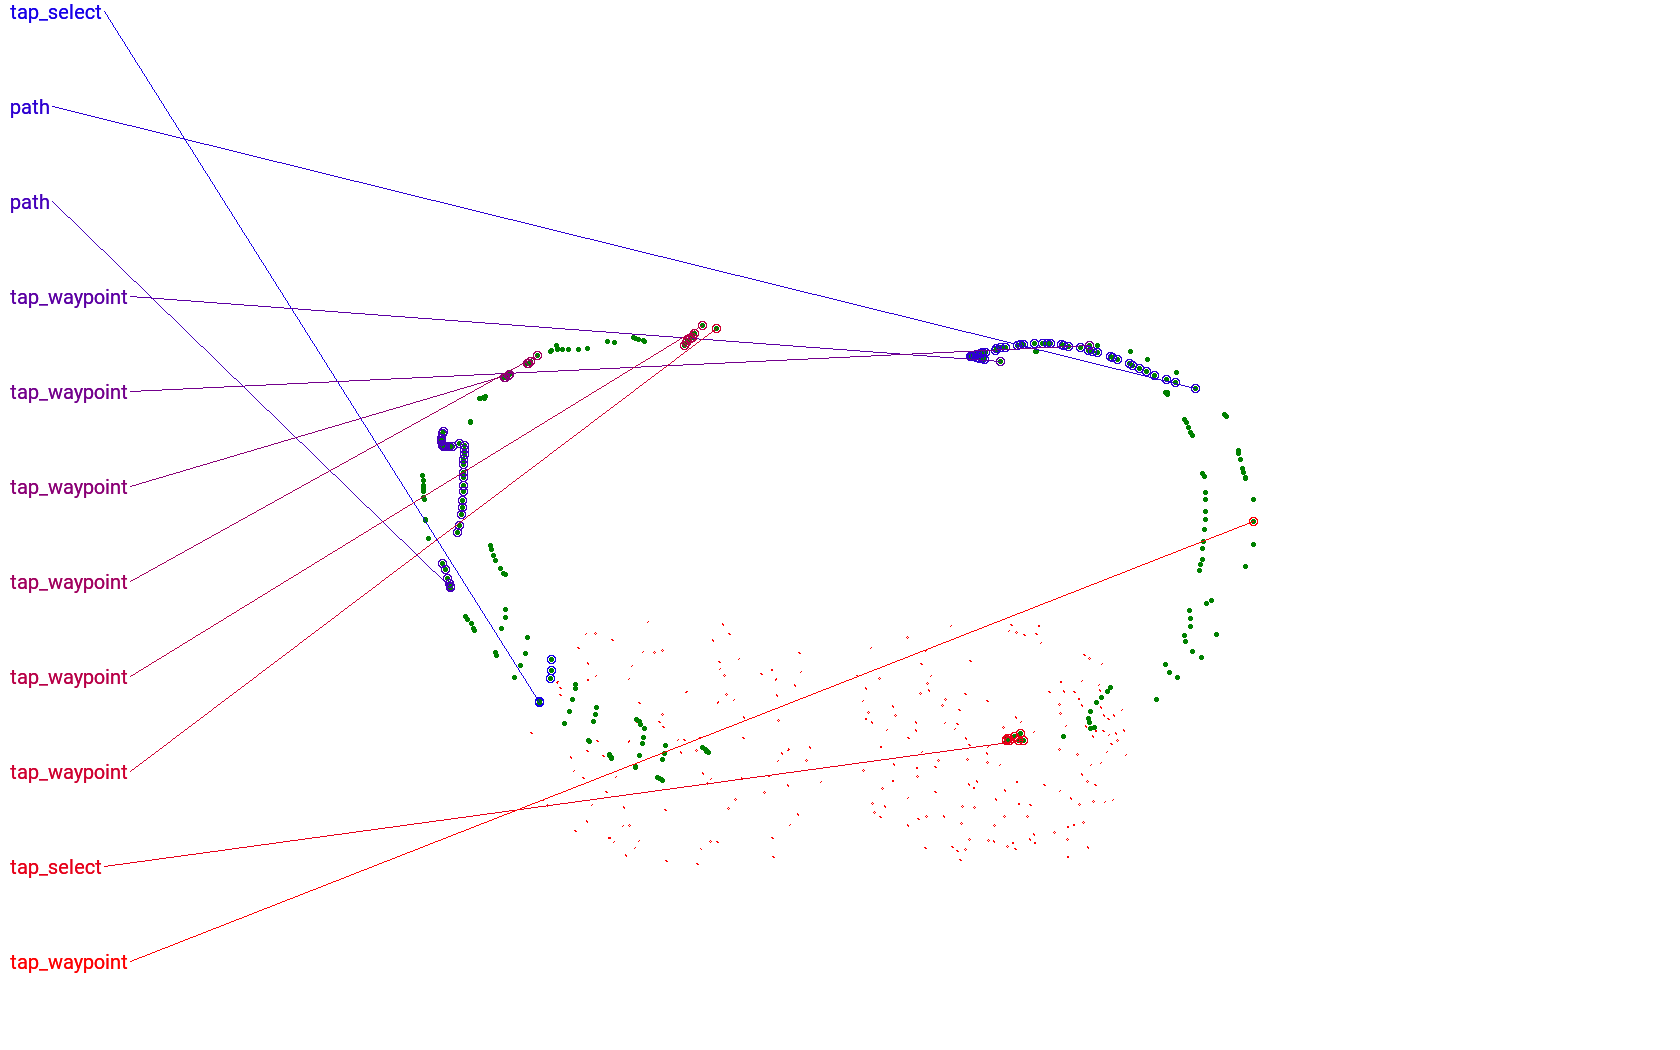
\includegraphics[width=\textwidth]{../../software/tool/test_pipeline/good_run/u10_c1000_t6/u10_c1000_t6_gestures.png}
	\caption{Result of a failed recognition, showing laddering between strokes and the system's guesses at the classes of each gesture.}
	\label{recognizer_fail_1}
\end{figure}

Also apparent in the output in figure \ref{recognizer_fail_1} are substantial gaps in the lines of points constituting the participant's gestures. 
These are locations where no points were recorded, likely due to stick-slip motion of the participant's finger, or a very light touch resulting in only intermittent detection of contact. 
The destuttering functionality in the earlier stages of the gesture pipeline was intended to eliminate these gaps, but it has fixed thresholds for how large the gap can be before the strokes are considered separate. 
Raising the thresholds so the gaps can be larger, in space or time, increases the risk that un-related gestures will be erroneously combined.

The stutter and interpolation-induced separation of the  participant's gestures into multiple strokes results in the detection of multiple gestures for a sequence that the participant intended as one gesture. 
On the right-hand gesture of figure \ref{recognizer_fail_1}, the tap selection gesture is followed by a tap-waypoint gesture, even though they should have been regarded as parts of a common gesture. 
Tap selection followed by tapping a waypoint, and then the end-of-command gesture would constitute a valid program, and so there is a possibility that stutter and laddering could result in valid, but undesired input. 

In addition to spuriously-detected gestures, stutter can cause gestures to not be detected. 
Lasso detection requires that the angle between the two ends of the gesture around its centroid be relatively small. 
If a section of the points at the beginning or end of the gesture is missing, the angle may be too open to detect correctly as a lasso. 
Obviously, a missing range of points anywhere else on the on the lasso could also break it into two separate arcs, neither of which would be sufficient to be considered a lasso on its own. 

In addition to light touches being regarded as intermittent contacts, another source of noise in the participant inputs was participants resting their fingers on the edges of the screen. 
This behavior was not common, and was generally coded by human coders as an action that was not intended to be an interaction with the screen, as if the user had accidentally bumped it. 
However, multitouch screens are prone to the Midas Touch problem, first seen in gaze-based UIs, where any contact on the screen (or any gaze direction) is considered an input for the computer \citep{jacob1990you}. 

A more subtle Midas Touch problem afflicted participant attempts to use group selection. 
There is a possible ambiguity between group selection gestures and single-robot drag gestures. 
If a user places their finger on a single robot, and drags a circle starting at that robot, the gesture is interpreted as a command to have the robot drive around in a circle.
However, if the user draws a circle around a group of robots, the gesture is interpreted as a lasso selection of that group of robots. 
Because the robots might be depicted as small on the screen, and so the user might not hit them precisely with a fingertip, it is possible to begin a robot drag gesture approximately a fingertip-width off the robot as well. 
However, this threshold lead to a great many of the participants attempts at box selection being interpreted as commands to drag a single robot through the group, and attempts at lasso selection to be interpreted as commands to have a single robot move around the outside of the group. 
This error also went the other way, where attempting to draw a figure, such as a box, in an area where there were already robots, would be recognized as a lasso selection, rather than a box.
Combined with stutter, the problem becomes even worse, as a single box selection could be broken up into multiple drag commands issued in rapid sequence. 
As selection finishes one command and begins another, each of these should be treated by the gesture translator as a complete and valid program, leaving a trail of chaos through the middle of the swarm. 

Similarly, multiple robots could have overlapping areas that would cause a tap between them to be regarded as a tap \emph{on} one of them, and so a selection of that robot.
As a result, it may become impossible to command an individual robot to move to a new position within the swarm, as tapping the target location would simply select a nearby robot. 

Lest it appear that all the gesture recognitions were fraught with error, in some cases the gesture detection worked perfectly and resulted in reasonable outputs, despite the fact that the participant input was collected well before the recognizers were written, and much of it was never selected for inclusion in the eventual gesture pipeline. 
For example, see \ref{recognizer_win}, where eight robot drag gestures were correctly detected.
 
 \begin{figure}
 	\centering
 	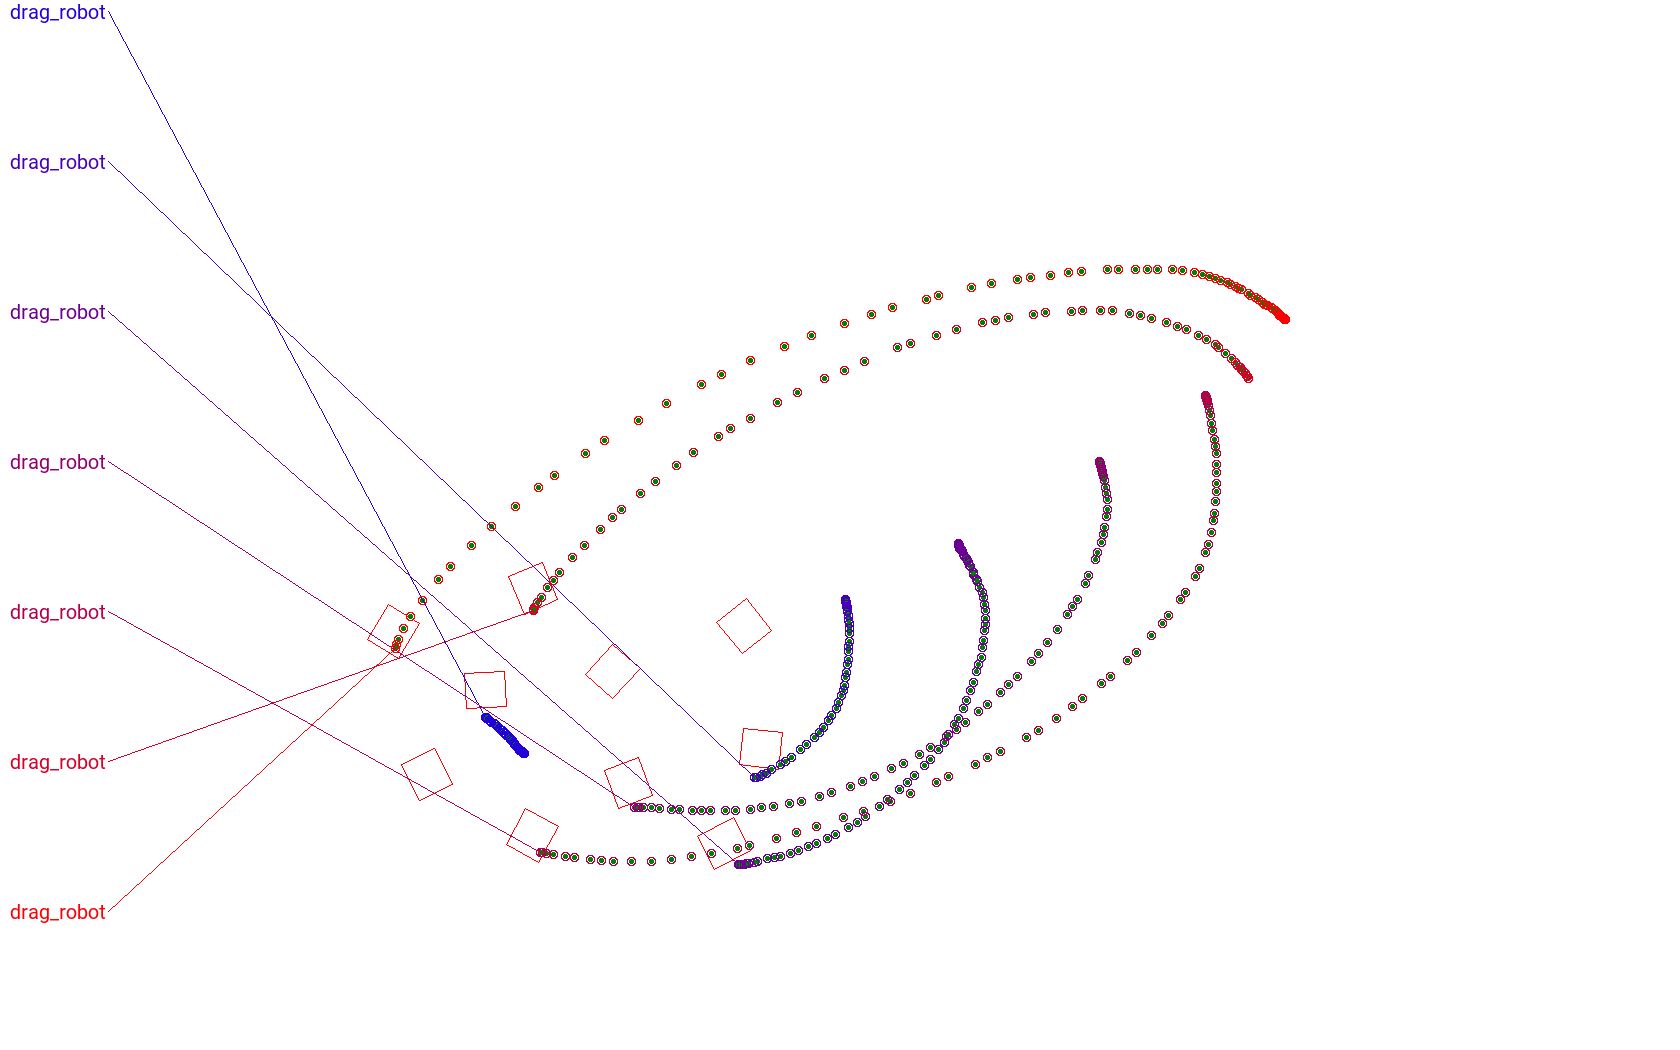
\includegraphics[width=\textwidth]{../../software/tool/test_pipeline/good_run/u8_c10_t10/u8_c10_t10_gestures.png}
 	\caption{Successful recognition of all gestures, moving eight of the robots to form a line with the other two. }
 	\label{recognizer_win}
 \end{figure}
 
In light of the gesture recognition's sensitivity to context, as well as the problems with stutter and light touches, this component of the system could be improved in a number of ways. 
The problem of combining intermittent contacts might be approached by searching across a gap in the direction of motion implied by the last few contacts, and allowing an approximate match for points on the opposite side of the gap, assuming the implied direction of motion was similar, and the gap crossing time was in approximate agreement with the calculated velocities between the last few points leading to the gap. 
Approaches such as this would require significant tuning of the parameters for the approximate matching, and so might work better for some users than others, as each user may have a different style of movement. 
Also, such approaches require a buffering of user input to allow the matching, and if the buffering becomes too long, will feel unresponsive or ``laggy'' to the user. 

Such a buffer might also be useful for deciding between two gestures that are ambiguous. 
For example, if a gesture might be a box select or might be a command to move a single robot from the edge of the swarm across it to the other edge, and the next command is a gesture from the swarm center to a location away from the swarm, then it is more likely that the intended command was box selection of the entire swarm and movement to the selected point, than movement of a single robot and then movement of another single robot to another point. 
However, even this is not certain, and so validation testing with users would be required to determine if making such a decision is always correct. 

Incorporating visual feedback to the user, particularly of selection, but also of what portion of a path was detected and would be used in the resulting command, may also mitigate these problems. 
If the user made a gesture intended as selection, but saw that no robots were selected, they could make an additional gesture to select before issuing their next command. 
Indeed, the entire list of detected gestures could be made visible to the user, perhaps as a stack along one edge of the screen, and edited by rearranging or deleting gestures before sending to the swarm. 
The current system dispatches gestures as they are recognized, and counts on the interpreter to convert them appropriately, which has some advantages in terms of responsiveness and simplicity, but disadvantages in terms of flexibility to the user and ability to undo gestures. 

\section{Translation Testing}

Translation testing is relatively straightforward. 
Either a sequence of gestures is in the order and of the types needed to be a valid ``sentence'' in the gesture language, or it is not. 
The recorded gesture sequences detected by the gesture detectors in the interface testing component, while they were being given the recorded participant input, were sent to a testing version of the gesture interpreter to see if they were detected as a valid program, or rejected. 

Four hundred forty-nine of the gestures resulting from the participant input were not accepted by the gesture translator. 
The primary causes of failure of a gesture set to be regarded as a valid input program for the gesture translator are the gesture set starting with a path (115 instances) or starting with a waypoint (81 instances). 
These problems arise any time that either the user did not begin a command with a selection, or the selection was mis-detected as a path. 
As discussed in the previous section, selections could be mis-detected as paths for a number of reasons, including stutter. 
Waypoints with no prior selection caused 15 failed translations, while paths with no prior selection caused 21 failures. 
In these cases, rather than the the gesture set starting with the waypoint or path, the waypoint or path occurs at some point within the gesture set, but has no preceding selection. 
The ultimate cause is similar to the cases where the gesture set starts with a waypoint or path, in that there is a waypoint or path that does not have a ``subject'' in the sentence for which the waypoint or path is the ``verb''.
In total, this class of errors accounts for 232 of the rejected gesture sets, or approximately 52\% of the rejections. 
This is not entirely unexpected, as the participants in the study were not required to perform selection gestures before waypoint or path gestures, and so many did not. 

Tap selection was designed to not start new gestures so that tap selections could be chained to select multiple robots, as discussed in section \ref{acceptable_cmd_seqs}.
However, as a result, alternating tap selections and commands would result in an error, as the tap selections that did not start the command would result in a translation error.
One approach to deal with this issue would be to allow a tap selection that occurs after an action other than a tap selection to cause the previous gestures to be passed off to the parser as a command, while leaving the existing tap selection in the queue. 
This behavior would be effective, but would require correction of the mis-recognition of waypoints as tap selects noted in the analysis of the gesture recognizers.
Taps near robots are classified as tap selections, so that users would not have to precisely hit the robots in order to select them. 
As previously noted, this can result in erroneous detections of taps intended as waypoints, but located near a robot, as tap selections. 
Additionally, stutter could cause a path dragged over robots to break up into what would be recognized as tap selections. 
If these tap selections resulted in the beginning of a new command and the execution of the previous gestures as a command, it could result in undesired movement of the robots. 

Drag robot operations do not chain, which is to say that while issuing a single drag robot gesture is accepted, multiple drag robot gestures in a row are not. 
It is likely a design oversight that drag robot commands are not treated as complete commands. 
After all, in the design language, they constitute both a selection and a motion command in a single gesture, with an implied subject, as in the English sentence "Go!". 
Were this oversight corrected, it might result in more of the participant gestures being accepted by the gesture translator. 
However, this problem interacts with the mis-recognition of lasso and box selection gestures as drag robot operations. 
Due to the common mis-recognition of box and lasso selections as drag robot gestures, many of these accepted gestures would be incorrect, and would result in undesired robot motion. 
Finally, drag robot gestures were frequently used with the intent that the entire swarm would be commanded to move, but the gesture recognizers treated them as intended to send a single robot along the dragged path. 
This caused some rejections of gesture sets because what the user intended as a selection and path was interpreted as a selection and a drag robot gesture, which is not regarded as a valid program because the selection has no meaning for the subsequent drag gesture. 

Thirty-five of the gesture sets had no gestures in them. The lack of gestures is not an error, and was caused by the participants not touching the screen during their interaction with the system. 

Thirty-seven of the gesture sets produced by running the participant gestures through the gesture detectors were acceptable to the gesture parser. 
Seventeen of them consisted of a single robot drag. 
Eleven of the accepted gesture sets were a set of tap selections followed by a sequence of waypoints, one more had a path instead of waypoints. 
Finally, six gesture sets were treated as disperse gestures, of which only one was actually intended by the user as a disperse and occurred in the disperse task. 
This is a design flaw that would probably best be solved by not treating the gestures as a strictly linear sequence, but only detecting a dispersal if all of the four or five strokes required to cause the detection overlap significantly. 
However, this would require implementation of a parser capable of dealing with simultaneity. 
The current parser is the Lark library, which, while a powerful parser, is intended for dealing with typical programming languages, which can be represented as a linear sequence of symbols \citep{LarkParser}. 
An alternate approach would be to include as part of gesture recognition a layer which detects sets of 4-5 overlapping strokes diverging from a central point, and replaces all of the strokes with a single gesture element, which takes the place of the simultaneous gestures in a linear representation of the gesture sequence. 

Ultimately, dealing with the issues in the gesture recognizers and gesture translation is an exercise in satisficing. 
The causes of many of the errors were primarily effects of design decisions made earlier in the development process in order to support participant behaviors from the user study. 
For example, the confusion between box selection and drag robot gestures was caused by the ability to select a robot by touching near it rather than on it, which was intended to make user interactions easier. 
Making the threshold for selection of a robot smaller would reduce these errors, but at the cost of making robot selection more difficult. 

%
%but treated as disperse u13 task 10, not disperse
%but treated as disperse u14 task 10, not disperse
%but treated as disperse u16 task 6, not disperse
%but treated as disperse u18 task 18, disperse
%but treated as disperse u19 task 4, not disperse
%but treated as disperse u4 task 12, not disperse

